%%%%%%%%%%%%%%%%%%%%%%%%%%%%%%%%%%%%%%%%%%%%%%%%%%%%%%%%%%%%%%%%%%%%%%%%%%%%%%%%
%                              Document Settings                               %
%%%%%%%%%%%%%%%%%%%%%%%%%%%%%%%%%%%%%%%%%%%%%%%%%%%%%%%%%%%%%%%%%%%%%%%%%%%%%%%%

\documentclass[a4paper,12pt]{article}
\usepackage[utf8]{inputenc}
%%%%%%%%%%%%%%%%%%%%%%%%%%%%%%%%%%%%%%%%%%%%%%%%%%%%%%%%%%%%%%%%%%%%%%%%%%%%%%%%
%                                   Margins                                    %
%%%%%%%%%%%%%%%%%%%%%%%%%%%%%%%%%%%%%%%%%%%%%%%%%%%%%%%%%%%%%%%%%%%%%%%%%%%%%%%%

\addtolength{\oddsidemargin}{-1.cm}
\addtolength{\textwidth}{2cm}
\addtolength{\topmargin}{-2cm}
\addtolength{\textheight}{3.5cm}

%%%%%%%%%%%%%%%%%%%%%%%%%%%%%%%%%%%%%%%%%%%%%%%%%%%%%%%%%%%%%%%%%%%%%%%%%%%%%%%%
%                                   Packages                                   %
%%%%%%%%%%%%%%%%%%%%%%%%%%%%%%%%%%%%%%%%%%%%%%%%%%%%%%%%%%%%%%%%%%%%%%%%%%%%%%%%

\usepackage[pdftex]{graphicx}	% Include graphics
\usepackage{float}				% Place floats inline, use the [H] placement
\usepackage{array}				% Additional tables features

\newcommand{\captionabove}[2][]{%
	\vskip-\abovecaptionskip
	\vskip+\belowcaptionskip
	\ifx\@nnil#1\@nnil
	\caption{#2}%
	\else
	\caption[#1]{#2}%
	\fi
	\vskip+\abovecaptionskip
	\vskip-\belowcaptionskip
}


%%%%%%%%%%%%%%%%%%%%%%%%%%%%%%%%%%%%%%%%%%%%%%%%%%%%%%%%%%%%%%%%%%%%%%%%%%%%%%%%
%                                   Document                                   %
%%%%%%%%%%%%%%%%%%%%%%%%%%%%%%%%%%%%%%%%%%%%%%%%%%%%%%%%%%%%%%%%%%%%%%%%%%%%%%%%

\begin{document}
	
	% Title page
	% Title page
	\begin{titlepage}
		\begin{center}
			
			% University Logo
			
\includegraphics[width=0.6\textwidth]{../images/up_logo.jpg}\\[2.0cm] 
			
			
			\textsc{\LARGE CS@UP Time Series Prediction}\\[1.0cm]
			
			
			\textsc{\Large Testing Document}\\[0.75cm]
			
			
			\textsc{\Large COS301 - Capstone Project}\\[0.75cm]
			
			
			% Students/Contributors Table
			\textbf{\huge \\ Team:}
			\huge NewGen Leaders \\
			\begin{flushright} \large
				Claudio Da Silva		\emph{u14205892} \newline
				Dedr\'e Olwage	    	\emph{u15015239} \newline
				Merrisa Joubert			\emph{u15062440} \newline
				Murray Le Roux	    	\emph{u15311644} \newline
			\end{flushright}
			\small Department of Computer Science, University of Pretoria \\ 
			
			
		\end{center}
		
		% Report Declaration		
		\noindent By submitting this document we confirm that we have read and are aware of the University of Pretoria's policy on academic dishonesty and plagiarism and we declare that the work submitted in this assignment is our own as delimited by the mentioned policies. We explicitly declare that no parts of this assignment have been copied from current or previous students' work or any other sources (including the internet), whether copyrighted or not. We understand that we will be subjected to disciplinary actions should it be found that the work we submit here does not comply with the said policies.
		
		\begin{center}
			
			% Fill page
			\vfill
			
			% Date
			{\large \today}
			
		\end{center}
		
	\end{titlepage}
    
    \tableofcontents
    
    \pagebreak
    
    % An overview of the Testing
    \section{Introduction}
    	
        %Specify the purpose of this SRS and the intended audience
        \subsection{Purpose}
        
        The purpose of this document is to show the level to which the system has been tested, as well as document problem areas and other concerns that may arise from testing. In the event that something in future may break, this document will be the proof that at the current time, the tests were indeed working.
        
        %Identify product by name, explain what the product will and will not do, describe the uses of the product including objectives, goals and benefits
        \subsection{Scope}
        
       The system will be used to enter, view, and edit student marks. It will include a prediction system that will use the student marks to make predictions on the outcomes of the students results at the end of the semester. These predictions will be used by lecturers to identify students who need extra help to pass the semester. The predictions may also be used to identify whether the teaching strategies of the lecturer are working as well as they expected it to. The system will allow students to view their marks and it will include an element of gamification that aims to improve student motivation. The ultimate goal of the system is to improve student results. The system also aims to improve the manner in which teaching assistants, tutors and lecturers record marks.
        
        \subsection{Definitions, Acronyms and Abbreviations}
        
       \begin{tabular}{ |c|c| } 
        	\hline
        	Term & Definition \\
        	\hline
        	NPM & The Node Package Manager, used to interact with node packages and scripts\\
        	\hline
        	CLI & A Command Line Interface, used to manipulate a program through command line\\
        	\hline
        	NYC & The CLI for the Istanbul code coverage module\\
        	\hline
        \end{tabular}
    
    \pagebreak
    
    % Explain the current testing framework in use
    \section{Testing framework}
    
    	% Describe the testing framework in place for the server
    	\subsection{Server}
    	
    		% Describe the chosen testign framework in place
	    	\subsubsection{The chosen testing framework}
	    	
	    	For server side, we make use of the jasmine testing framework for nodeJS. We also use Istanbul in order to check for test coverage, via their CLI, NYC.
	    	
	    	% Explain how to run the tests for the that framework
	        \subsubsection{How to run the tests}
	        
	        To run the tests, simply go to the root folder of the application, open up a command line instance and type, "npm test".
	        
	        % Explain the current system of automated testing and how to use and view it
	        \subsubsection{Automated testing overview}
	        
	        Tests are run on a GitHub push basis using the Travis Continuous Integration tool. A weekly check is also run to ensure everything stays in order. Code Climate is then used to determine the quality of code being written, as well as document the level of code that is covered, as determined by Istanbul.
	        
	    	% Describe the testing framework in place for the client
	    \subsection{Web Client}
	    
	    % Describe the chosen testign framework in place
	    \subsubsection{The chosen testing framework}
	    
    	For client side, we make use of the jasmine testing framework for nodeJS. We however make use of Karma to run jasmine, as a more Angular friendly approach. Protractor is also used to run tests that simulate user input.
	    
	    % Explain how to run the tests for the that framework
	    \subsubsection{How to run the tests}
	    
	     To run the tests, simply go to the root folder of the application, open up a command line instance and type, "npm test" or alternatively "ng test".
	    
	    % Explain the current system of automated testing and how to use and view it
	    \subsubsection{Automated testing overview} 
	    
	    Tests are run on a GitHub push basis using the Travis Continuous Integration tool. A weekly check is also run to ensure everything stays in order.
      
    \pagebreak 
    % List the tests performed on the system
    \section{System tests}
    
    	% List the unit tests which test the functions in the system
    	\subsection{Unit tests}
    	
    		\subsubsection{Server}
    		
   			\begin{tabular}{ |c|c|c| } 
    			\hline
    			Test number & Test overview & Test result \\
    			\hline
    			1 & Forgot password sends right URL & Passing\\
    			\hline
    			2 & GetUsers returns a list of users & Passing\\
    			\hline
    			3 & Validation fails if username is empty & Passing\\
    			\hline
    			4 & Validation fails if password is empty & Passing\\
    			\hline
    			5 & Validation fails if email is empty & Passing\\
    			\hline
    			6 & Correct password validated & Passing\\
    			\hline
    			7 & Incorrect password invalidated & Passing\\
    			\hline
    			8 & Invalidate incorrect password casing & Passing\\
    			\hline
    			9 & Invalidate extra spaces in password & Passing\\
    			\hline
    			10 & Authenticates if token valid & Passing\\
    			\hline
    			11 & Sets the user in the request object & Passing\\
    			\hline
    			12 & Unauthorized access if JSON invalid & Passing\\
    			\hline
    			13 & Unauthorized access if not encrypted & Passing\\
    			\hline
    			14 & Unauthorized access if token expired & Passing\\
    			\hline
    			15 & Unauthorized access if IP does not match & Passing\\
    			\hline
    			16 & Unauthorized access if token not set & Passing\\
    			\hline
    			17 & Generate token should return encrypted token & Passing\\
    			\hline
    			18 & Encrypt/decrypt should work on data & Passing\\
    			\hline
    			19 & GetSalt should return same length salt & Passing\\
    			\hline
    			20 & GetSalt should append salt to hash & Passing\\
    			\hline
    			21 & GetSalt should compute same hash with same data & Passing\\
    			\hline
    			22 & GenerateResetToken should be URL safe & Passing\\
    			\hline
    			23 & GenerateResetToken should be 20 characters long & Passing\\
    			\hline
   				24 & Auth should deny authorisation if not admin and no permissions & Passing\\
    			\hline
   				25 & Auth should grant authorisation if admin and no other permissions & Passing\\
    			\hline
   				26 & Auth should deny if user has permissions but not for right module & Passing\\
    			\hline
   				27 & Auth should grant auth if user has permissions for right module & Passing\\
    			\hline
   				28 & Auth should grant auth if user has higher permissions than needed & Passing\\
    			\hline
   				29 & Auth should deny edit if user has view permissions for module only & Passing\\
    			\hline
   				30 & Auth should deny authorisation if moduleCode not given & Passing\\
    			\hline
   				31 & AdminOnly should deny authorisation if not admin & Passing\\
    			\hline
   				32 & AdminOnly should grant authorisation if admin & Passing\\
    			\hline
    			33 & GetModules should resolve all the modules & Passing\\
    			\hline
    			34 & GetModules should call findOne with module code & Passing\\
    			\hline
    			35 & GetModules should resolve with module & Passing\\
    			\hline
    		\end{tabular}
    		
    		\subsubsection{Web Client}
    		
   			\begin{tabular}{ |c|c|c| } 
    			\hline
    			Test number & Test overview & Test result \\
    			\hline
   				1 & addUsers should call api post with correct args & Passing\\
    			\hline
   				2 & addUsers should return a message observable & Passing\\
    			\hline
   				3 & addUser should call api post with correct args & Passing\\
    			\hline
   				4 & addUser should return a message observable & Passing\\
    			\hline
   				5 & grid API is not available until `detectChanges` & Passing\\
    			\hline
   				6 & grid API is available after `detectChanges` & Passing\\
    			\hline
   				7 & select all button selects all rows & Passing\\
    			\hline
   				8 & Api Service should call httpGet with correct arguments & Passing\\
    			\hline
   				9 & Api Service should call httpDelete with correct arguments & Passing\\
    			\hline
   				10 & Api Service should call httpPut with correct arguments & Passing\\
    			\hline
   				11 & Api Service should call httpPost with correct arguments & Passing\\
    			\hline
   				12 & Api Service should append authToken to headers & Passing\\
    			\hline
   				13 & Api Service should set new AuthToken & Passing\\
    			\hline
   				14 & getAssessmentsByModule should call api get with correct args & Passing\\
    			\hline
   				15 & getAssessmentsByModule should return array of assessments & Passing\\
    			\hline
   				16 & AddAssessment should call api put with correct args & Passing\\
    			\hline
   				17 & AddAssessment should return a message observable & Passing\\
    			\hline
   				18 & AddQuery should call api post with correct args & Passing\\
    			\hline
   				19 & AddQuery should return a message observable & Passing\\
    			\hline
   				20 & getMarksByAssessment should call api get with correct args & Passing\\
    			\hline
   				21 & getMarksByAssessment should return a marks array & Passing\\
    			\hline
   				22 & addFinalMarksToAssessment should call api post with correct args & Passing\\
    			\hline
   				23 & addFinalMarksToAssessment should return a response message & Passing\\
    			\hline
   				24 & addModule should call api post with correct args & Passing\\
    			\hline
   				25 & addModule should return a message observable & Passing\\
    			\hline
   				26 & assignHOD should call api put with correct args & Passing\\
    			\hline
   				27 & assignHOD should return a message observable & Passing\\
    			\hline
   				28 & deleteModule should call api del with correct args & Passing\\
    			\hline
   				29 & deleteModule should return a message observable & Passing\\
    			\hline
   				30 & enrollStudents should call api del with correct args & Passing\\
    			\hline
   				31 & enrollStudents should return a message observable & Passing\\
    			\hline
   				32 & getAllModules should call api get with correct args & Passing\\
    			\hline
   				33 & getAllModules should return array of modules & Passing\\
    			\hline
   				34 & getModule should call api get with correct args & Passing\\
    			\hline
   				35 & getModule should return array of modules & Passing\\
    			\hline
   				36 & getStudentsByModule should call api get with correct args & Passing\\
    			\hline
   				37 & getStudentsByModule should return array of assessments & Passing\\
    			\hline
   				38 & isAdmin should return true if user is admin & Passing\\
    			\hline
   				39 & isAdmin should return false if user is not admin & Passing\\
    			\hline
   				40 & isStaffMember should return false if only student & Passing\\
    			\hline
   				41 & isStaffMember should return true if staff member for any module & Passing\\
    			\hline
   				42 & getPermissionForModule should return 0 if no permissions for module & Passing\\
    			\hline
   				43 & getPermissionForModule should return correct permission if student & Passing\\
    			\hline
 				44 & getPermissionForModule should return correct permission if admin & Passing\\
    			\hline
  				45 & isStudent should return true if student & Passing\\
    			\hline
  				46 & isStudent should return false if staff member & Passing\\
    			\hline
  				47 & isStudent should return false if no permissions for module & Passing\\
    			\hline
    			48 & isStaffMemberForModule should return false if student & Passing\\
    			\hline
    		\end{tabular}
    	
    	% List the integration tests which test compatability between modules
        \subsection{Integration tests}
        
        	\subsubsection{Server}
        	
        	N/A
        	
        	\subsubsection{Web Client}
        
        		
        	\begin{tabular}{ |c|c|c| } 
        		\hline
        		Test number & Test overview & Test result \\
        		\hline
        		1 & App Component was successfully created & Passing\\
        		\hline
       			2 & Authorization Guard was successfully created & Passing\\
        		\hline
        		3 & Authorization Service was successfully created & Passing\\
        		\hline
        		4 & UsersApi Service was successfully created & Passing\\
        		\hline
				5 & AdminMarksInterface Component was successfully created & Passing\\
        		\hline
       			6 & AdminQueryComponent was successfully created & Passing\\
        		\hline
        		7 & AssignmentsComponent was successfully created & Passing\\
        		\hline
        		8 & GradingComponent was successfully created & Passing\\
        		\hline
        		9 & LeaderboardComponent was successfully created & Passing\\
        		\hline
        		10 & MarksComponent was successfully created & Passing\\
        		\hline
        		11 & NavbarComponent was successfully created & Passing\\
        		\hline
        		12 & RedComponentComponent was successfully created & Passing\\
        		\hline
        		13 & StudentDashComponent was successfully created & Passing\\
        		\hline
        		14 & StudentQueryComponent was successfully created & Passing\\
        		\hline
        		15 & WeightingsComponent was successfully created & Passing\\
        		\hline
        		16 & Api Service was successfully created & Passing\\
        		\hline
     			17 & AssessmentsApi Service was successfully created & Passing\\
        		\hline
        		18 & AssessmentsApiService was successfully created & Passing\\
        		\hline
        		19 & ModulesApiService was successfully created & Passing\\
        		\hline
        	\end{tabular}
        
        % List the functional/system test which test functionality between containers, and overall working of the system
        \subsection{Functional/system tests}
	
		Human tested only
		
	\pagebreak
	\section{Usability Testing}
	
	\begin{figure}[H]
		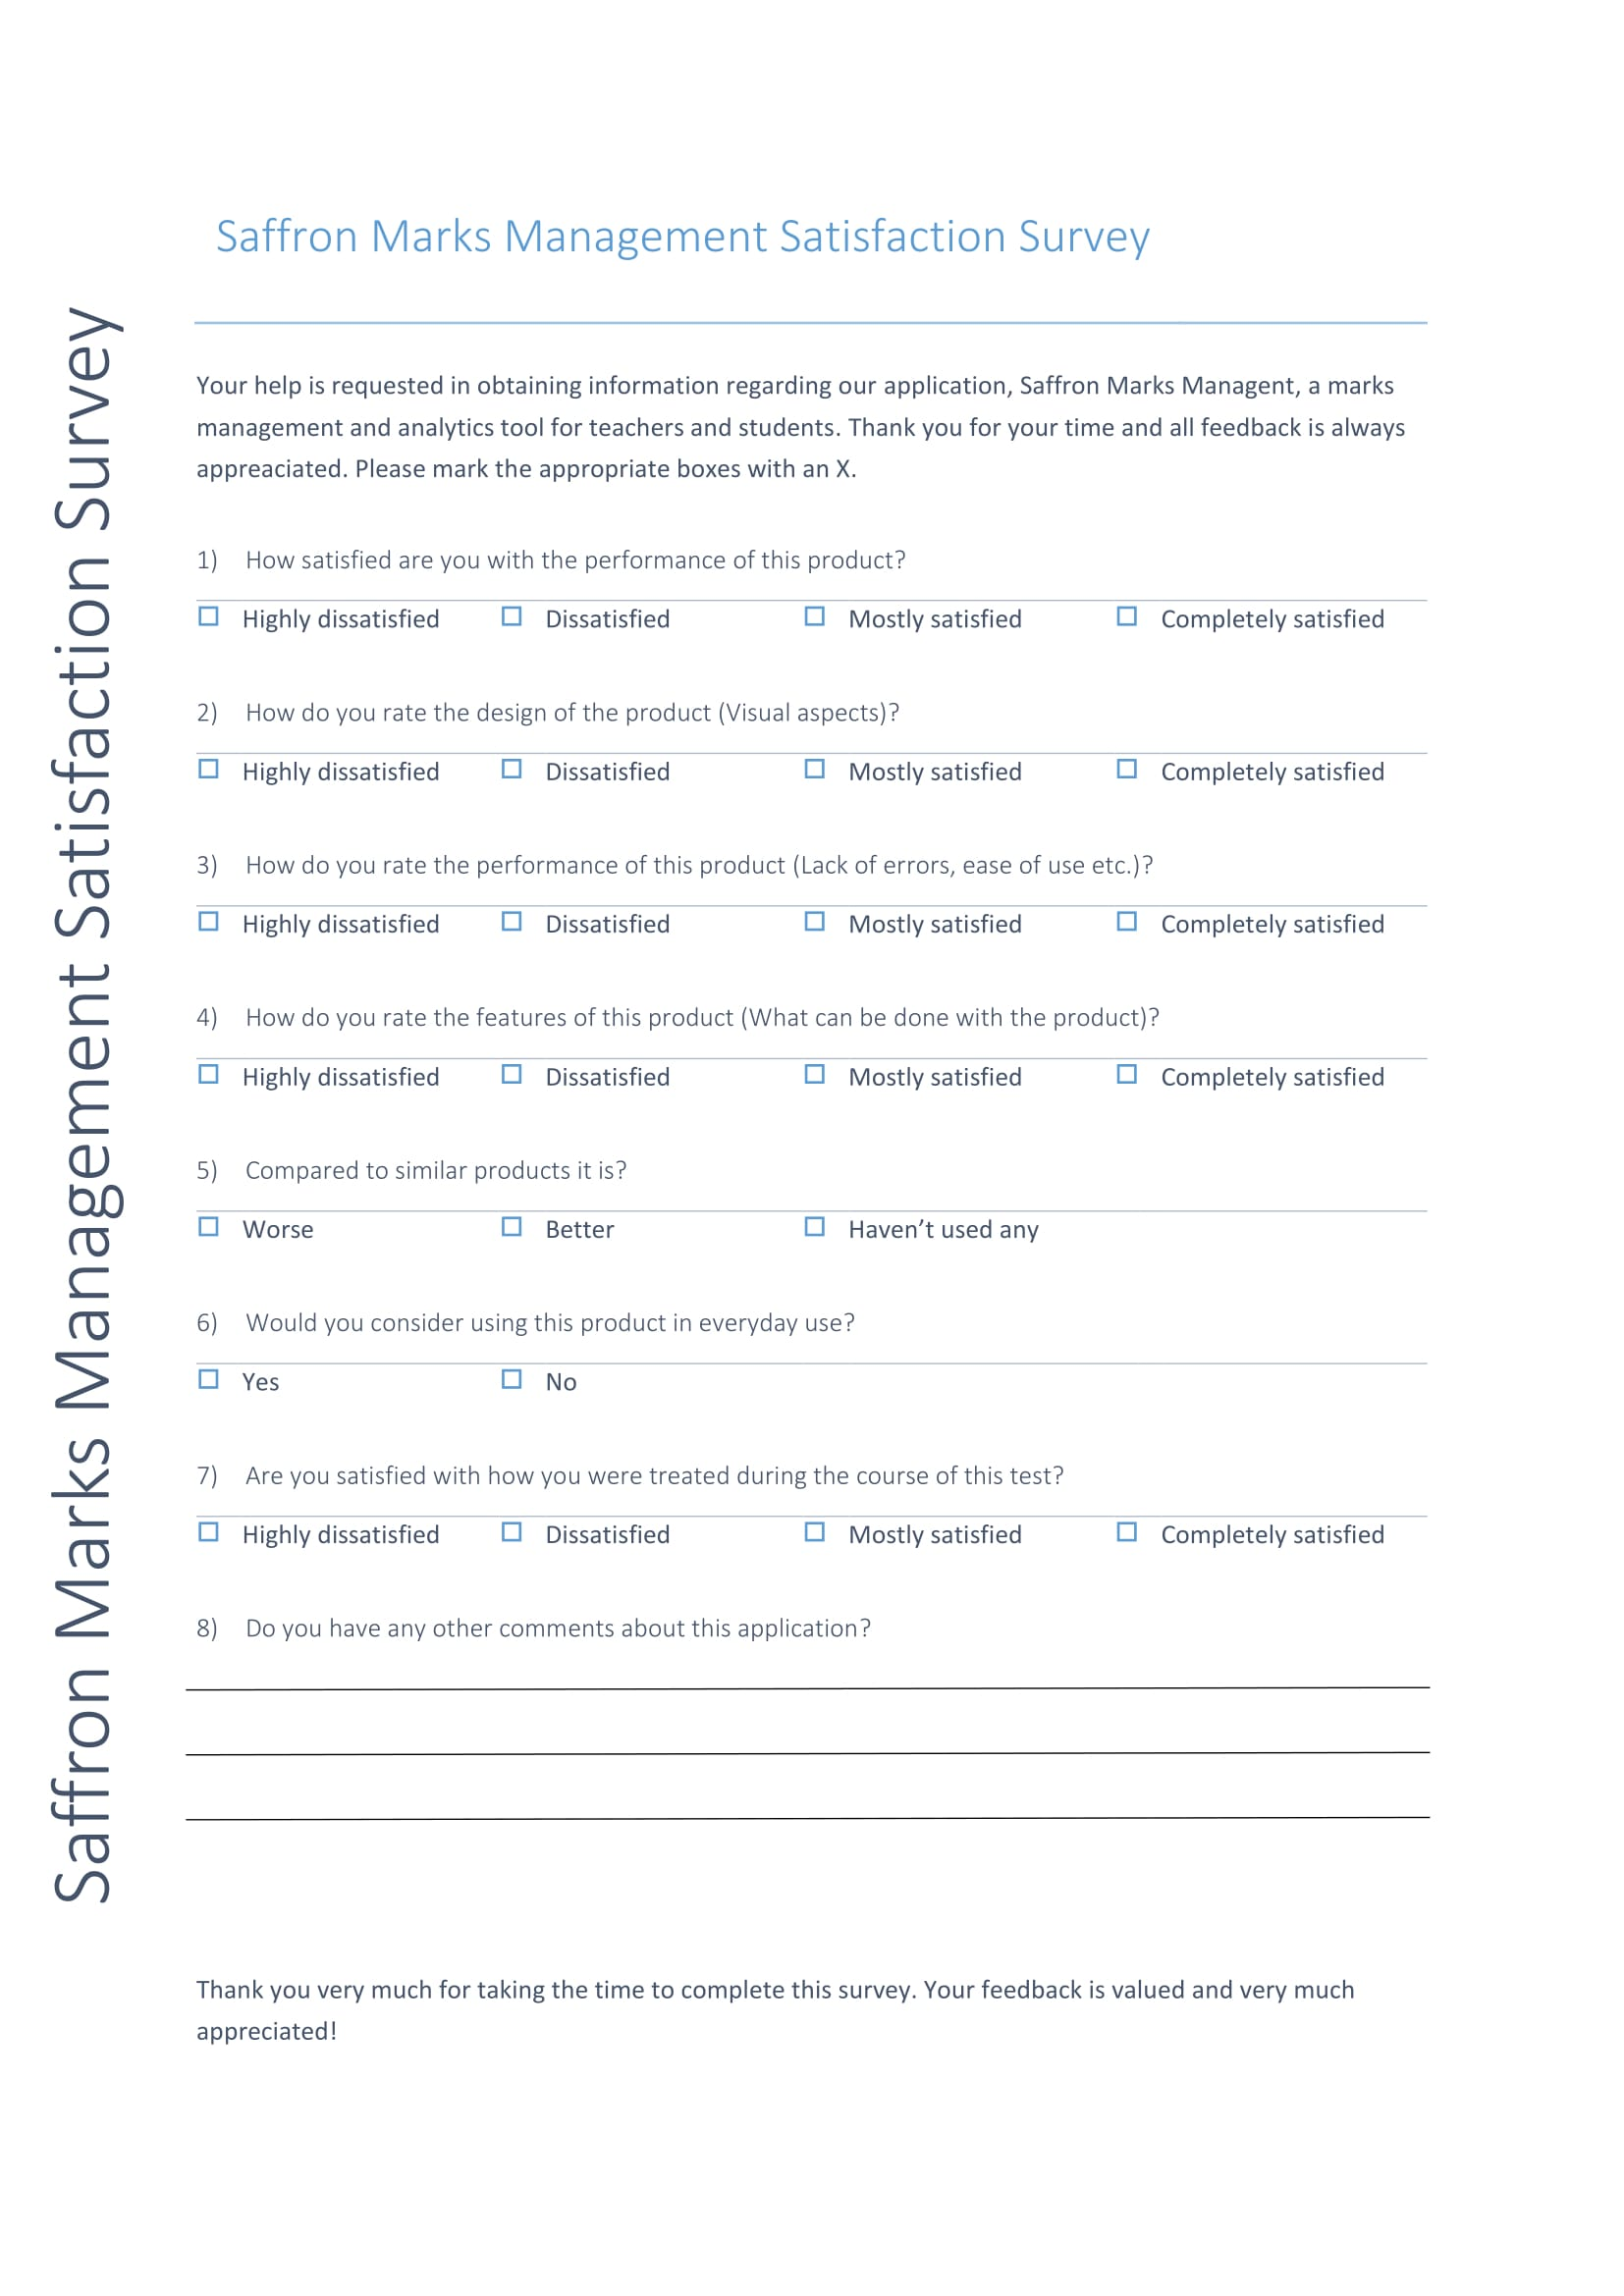
\includegraphics[width=\linewidth]{../images/Saffron_marks_survey.jpg}
		\captionabove{Usability test survey}
		\label{fig:Usability test survey}
	\end{figure}

	The following usability test was performed using six users, of which one was a lecturer, two were currently teaching assistants and the remaining three were enrolled students.\\
	
	\textbf{The results for the usability test are displayed below:}
	
	\begin{table}[H] \centering \captionabove{Usability Question 1-4} \label{my-label} \begin{tabular}{|l|c|} \hline \multicolumn{1}{|c|}{\textbf{Question}} & \multicolumn{1}{l|}{\textbf{Average user rating}} \\ \hline How satisfied are you with the consistency of this product? & 2.5 \\ \hline How do you rate the design of the product (Visual aspects)? & 2 \\ \hline \begin{tabular}[c]{@{}l@{}}How do you rate the performance of this product\\ (Lack of errors, ease of use etc.)?\end{tabular} & 2 \\ \hline \begin{tabular}[c]{@{}l@{}}How do you rate the features of this product\\ (What can be done with the product to what is expected)?\end{tabular} & 2.5 \\ \hline \end{tabular} \end{table}
	
	\textbf{User rating rubric:\\\\}
	Highly dissatisfied = 1\\
	Dissatisfied = 2\\
	Mostly satisfied = 3\\
	Completely satisfied = 4\\\\
	\textbf{The bar graph for the results is displayed below:}\\
	
	\begin{figure}[H]
		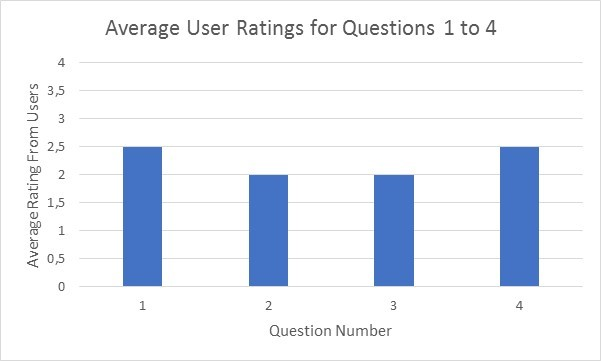
\includegraphics[width=\linewidth]{../images/average_user_ratings.jpg}
		\captionabove{Usability test bar graph}
		\label{fig:Usability test bar graph}
	\end{figure}
	
	\textbf{The remaining questions of the usability test are shown below:\\}
	
	\begin{table}[H] \centering \captionabove{Usability Question 5 \& 6} \label{my-label} \begin{tabular}{|l|l|l|l|l|l|l|} \hline Question & User1 & User2 & User3 & User4 & User5 & User6 \\ \hline Compared to similar products it is? & Worse & Worse & \begin{tabular}[c]{@{}l@{}}Worse\end{tabular} & \begin{tabular}[c]{@{}l@{}}Worse\end{tabular} & Worse & Worse \\ \hline \begin{tabular}[c]{@{}l@{}}Would you consider using this product \\ in everyday use?\end{tabular} & No & No & No & No & Yes & No \\ \hline \end{tabular} \end{table}
	
	\subsubsection{Comments}
	
	Some of the comments included:
	\begin{itemize}
		\item The biggest problem with the system was that it was not production ready enough to compare with other current systems
		\item Colors seem too inconsistent, also material should be used more across the application.
		\item Users liked the ability to be able to receive notifications of marks when available
	\end{itemize}
	
	\subsubsection{Conclusion}
	Overall the users felt that the worst problem was that the system did not feel production ready enough. A concern that users had is that the system looked too inconsistent at times, to which the colour scheme was adjusted and fixed. The users found the system intuitive, but said that not enough features were available to make it easily more usable than the paid counterparts. The material elements were a hit with the testers, and have been slowly introduced as the material library for Angular2 has expanded. Users could see themselves using it on a regular basis if more features were added. All the user opinions and data was collected from the usability survey provided to the users as well as a short interview.
	
	\pagebreak
	\section{Testing release log}
	
	\begin{itemize}
		\item \textbf{Server}
		\begin{itemize}
			\item
				\begin{tabular}{ |c|c|c| } 
					\hline
					Date & Number of tests & Number of passing tests \\
					\hline
					2017/07/28 & 23 & 23\\
					\hline
					2017/08/25 & 23 & 23\\
					\hline
					2017/10/12 & 35 & 35\\
					\hline
				\end{tabular}
		\end{itemize}
 	\end{itemize}
 
	\begin{itemize}
 		\item \textbf{Client}
 		\begin{itemize}
 			\item
 			\begin{tabular}{ |c|c|c| } 
 				\hline
 				Date & Number of tests & Number of passing tests \\
 				\hline
 				2017/07/28 & 3 & 3\\
 				\hline
 				2017/08/25 & 3 & 3\\
 				\hline
 				2017/10/12 & 67 & 67\\
 				\hline
 			\end{tabular}
 		\end{itemize}
 	\end{itemize}  
   
    \section{Appendixes}
    
    \section{Index}
    \pagebreak  

\end{document}
